\pdfoutput=1
\documentclass[12pt,a4paper]{article}
\usepackage[utf8]{inputenc}
\usepackage{amsmath}
\usepackage{amsfonts}
\usepackage{amssymb}
\usepackage{amsthm}
\usepackage[margin=0.7in]{geometry}
\usepackage{graphicx}
\usepackage{todonotes}
\usepackage{natbib}
\usepackage{url}
\usepackage[boxruled,vlined,linesnumbered]{algorithm2e}
\usepackage{caption}
\usepackage{subcaption}
\usepackage{lineno}
\usepackage{tcolorbox}
\usepackage{caption}
\usepackage{hyperref}
\usepackage{marginnote}
\AtBeginDocument{\let\textlabel\label}
\hypersetup{colorlinks=true,linkcolor=black,citecolor=black,filecolor=black,urlcolor=black}


\author{Jonathan Rosenblatt \\ Ben Gurion University}

%% OPTIONAL MACRO DEFINITIONS
\renewcommand*{\marginfont}{\scriptsize }

\newcommand{\reals}{\mathbb{R}} % the set of real numbers
\newcommand{\argmin}[2]{\textstyle{\mathop{argmin}_{#1}}\set{#2}} % The argmin operator
\newcommand{\argmax}[2]{\textstyle{\mathop{argmax}_{#1}}\set{#2}} % The argmin operator
\newcommand{\manifold}{\mathcal{M}} % A manifold.
\newcommand{\project}{\hookrightarrow} % The orthogonal projection operator.
\newcommand{\projectMat}{H} % A projection matrix.
\newcommand{\encode}{E} % a linear encoding matrix
\newcommand{\decode}{D} % a linear decoding matrix
\DeclareMathOperator{\Tr}{Tr}
\newcommand{\set}[1]{\{ #1 \}} % A set
\newcommand{\setII}[1]{\left\{ #1 \right\}} % A set
\newcommand{\rv}[1]{\mathbf{#1}} % A random variable
\newcommand{\x}{\rv x} % The random variable x 
\newcommand{\y}{\rv y} % The random variable x 
\newcommand{\U}{\rv u} % The random variable x 
\newcommand{\T}{\rv t} % The random variable x 
\newcommand{\X}{\rv X} % The random variable x 
\newcommand{\Y}{\rv Y} % The random variable y
\newcommand{\expect}[1]{\mathbf{E}\left[ #1 \right]} % The expectation operator
\newcommand{\expectg}[2]{\mathbf{E}_{\rv{#1}}\left[ \rv{#2} \right]} % An expectation w.r.t. a particular random variable.
\newcommand{\expectn}[1]{\mathbb{E}\left[#1\right]} % The empirical expectation
\newcommand{\cov}[1]{\mathbf{Cov} \left[ #1 \right]} % The expectation operator
\newcommand{\var}[1]{\mathop{Var} \left[ #1 \right]} % The expectation operator
\newcommand{\covn}[1]{\mathbb{Cov} \left[ #1 \right]} % The expectation operator
\newcommand{\gauss}[1]{\mathcal{N}\left(#1\right)} % The gaussian distribution
\newcommand{\cdf}[2]{F_{#1} (#2)} % The CDF function
\newcommand{\survive}[2]{S_{#1} (#2)} % The survival function
\newcommand{\hazard}[2]{h_{#1} (#2)} % The survival function
\newcommand{\cuhazard}[2]{H_{#1} (#2)} % The survival function
\newcommand{\cdfn}[2]{\mathbb{F}_{#1}(#2)} % The empirical CDF function
\newcommand{\icdf}[2]{F_\rv{#1}^{-1} (#2)} % The invecrse CDF function
\newcommand{\icdfn}[2]{\mathbb{F}^{-1}_{#1}(#2)} % The inverse empirical CDF function
\newcommand{\pdf}[2]{p_{#1} (#2)} % The CDF function
\newcommand{\prob}[1]{P\left( #1 \right)} % the probability of an event
\newcommand{\dist}{P} % The proabaiblity distribution
\newcommand{\density}{p}
\newcommand{\entropy}{H} % entropy
\newcommand{\mutual}[2]{I\left(#1;#2\right)} % mutual information
\newcommand{\norm}[1]{\Vert #1 \Vert} % The norm operator
\newcommand{\normII}[1]{\norm{#1}_2} % The norm operator
\newcommand{\normI}[1]{\norm{#1}_1} % The norm operator
\newcommand{\normF}[1]{\norm{#1}_{Frob}} % The Frobenius matrix norm
\newcommand{\ones}{\textbf{1}} % Vector of ones.
\newcommand{\lik}{\mathcal{L}} % The likelihood function
\newcommand{\loglik}{L} % The log likelihood function
\newcommand{\loss}{l} % A loss function
\newcommand{\lossII}{\prescript{}{2}{l}} % A loss function
\newcommand{\risk}{R} % The risk function
\newcommand{\riskn}{\mathbb{R}} % The empirical risk
\newcommand{\riskII}{\prescript{}{2}{R}} % The empirical risk
\newcommand{\risknII}{\prescript{}{2}{\mathbb{R}} } % The empirical risk
\newcommand{\noisen}{\mathbb{G}} % The empirical noise process
\newcommand{\deriv}[2]{\frac{\partial #1}{\partial #2}} % A derivative
\newcommand{\hyp}{f} % A hypothesis
\newcommand{\hypclass}{\mathcal{F}} % A hypothesis class
\newcommand{\hilbert}{\mathcal{H}}
\newcommand{\rkhs}{\hilbert_\kernel} % A hypothesis class
\newcommand{\normrkhs}[1]{\norm{#1}_{\rkhs}} % the RKHS function norm
\newcommand{\rank}{q} % A subspace rank.
\newcommand{\dimy}{K} % The dimension of the output.
\newcommand{\latent}{\rv{s}} % latent variables matrix
\newcommand{\latentn}{S} % latent variables matrix
\newcommand{\loadings}{A} % factor loadings matrix
\newcommand{\rotation}{R}  % rotation matrix
\newcommand{\similaritys}{\mathfrak{S}} % a similarity graph
\newcommand{\similarity}{s} % A similarity measure.
\newcommand{\dissimilarity}{d} % A dissimilarity measure.
\newcommand{\dissimilaritys}{\mathfrak{D}} % a dissimilarity graph
\newcommand{\scalar}[2]{\left< #1,#2 \right>} % a scalar product
\newcommand{\aka}{{a.k.a.\ }}
\newcommand{\Aka}{{A.k.a.\ }}









\theoremstyle{plain}
\newtheorem{theorem}{Theorem}[section]
\newtheorem*{theorem*}{Theorem}
\newtheorem{lemma}{Lemma}[section]
\newtheorem*{lemma*}{Lemma}
\newtheorem{prop}{Proposition}[section]
\newtheorem{cor}{Corollary}[section]


\theoremstyle{definition}
\newtheorem{definition}{Definition}
\newtheorem{remark}{Remark}
%\newtheorem{think}{Gedankenexperiment}
%\newtheorem*{think}{Think about it \faLightbulbO}

\newtheorem{example}{Example}

\newenvironment{think}
	{
		\bigskip
		\begin{tcolorbox}
		\paragraph{Think about it.}
	}{
		\end{tcolorbox}
}

\newenvironment{extra}
{
	\bigskip
	\begin{tcolorbox}
		\paragraph{Extra Information.}
	}{
	\end{tcolorbox}
}



% Custom commands

\newcommand{\naive}{na\"{\i}ve }
\newcommand{\Naive}{Na\"{\i}ve }
\newcommand{\andor}{and\textbackslash or }
\newcommand{\erdos}{Erd\H{o}s }
\newcommand{\renyi}{R\`enyi }


\title{Dimensionality Reduction}


\begin{document}

\maketitle

\begin{example}[BMI]
	\label{ex:bmi}
	Consider the heights and weights of a sample of individuals. 
	The data may seemingly reside in $2$ dimensions but given the height, we have a pretty good guess of a person's weight, and vice versa. 
	We can thus state that heights and weights are not really two dimensional, but roughly lay on a $1$ dimensional subspace of $\reals^2$. 
\end{example}


\begin{example}[IQ]
	\label{ex:iq}
	Consider the correctness of the answers to a questionnaire with $p$ questions. 
	The data may seemingly reside in a $p$ dimensional space, but assuming there is such a thing as ``skill'', then given the correctness of a person's reply to a subset of questions, we have a good idea how he scores on the rest. 
	Put differently, we don't really need a $200$ question questionnaire-- $100$ is more than enough.
	If skill is indeed a one dimensional quality, then the questionnaire data should organize around a single line in the $p$ dimensional cube. 
\end{example}


\begin{example}[Blind signal separation]
	\label{ex:blind-signal}
	Consider $n$ microphones recording an individual. 
	The digitized recording consists of $p$ samples. 
	Are the recordings really a shapeless cloud of $n$ points in $\reals^p$?
	Since they all record the same sound, one would expect them to arrange around a single 
\end{example}
		
	






\section{Enter the King: Principal Component Analysis}
\label{sec:pca}

\emph{Principal Component Analysis} (PCA) is such a basic technique, it has been rediscovered and renamed independently in many fields. 
It can be found under the names of 
\emph{
	Discrete Karhunen–Loève Transform; 
	Hotteling Transform; 
	Proper Orthogonal Decomposition (POD); 
	Eckart–Young Theorem; 
	Schmidt–Mirsky Theorem;  
	Empirical Orthogonal Functions; 
	Empirical Eigenfunction Decomposition;  
	Empirical Component Analysis;  
	Quasi-Harmonic Modes;  
	Spectral Decomposition;  
	Empirical Modal Analysis}, 
and possibly more\footnote{\url{http://en.wikipedia.org/wiki/Principal_component_analysis} }.
The many names are quite interesting as they offer an insight into the different problems that led to PCA's (re)discovery.


Return to the BMI problem in Exampl~\ref{ex:bmi}.
Assume you now wish to give each individual a ``size score'', that is a \textbf{linear} combination of height and weight: PCA does just that. 
It returns the linear combination that has the largest variability, i.e., the combination which best distinguishes between individuals. 

The variance maximizing motivation above was the one that guided Hotelling \citet{hotelling1933analysis}.
But $30$ years before him, \citet{pearson1901liii} derived the same procedure with a different motivation in mind. 
Pearson was also trying to give each individual a score. 
He did not care about variance maximization, however. 
He simply wanted a small set of coordinates in some (linear) space that approximates the original data well. 
As it turns out, the best linear-space approximation of $X$ is also the variance maximizing one. 
More precisely: the \emph{sequence} of $1,\dots,p$ dimensional linear spaces that best approximate $X$, is exactly the sequence of $1,\dots,p$ dimensional scores, that best separate between the $n$ samples. 
Pearson and Hotelling (among others) thus arrived to the exact same solution, with different motivations. 






\subsubsection{Bi Plot}
\label{sec:bi_plot}
The \emph{Bi-Plot} shows the two first scores of the original data points.
These scores are known as the \emph{Principal Componets} (PCs). \marginnote{Principal Components}
The contribution of each original variable to each PC, is called the \emph{Loadings}.
The plot also shows the contribution of each of the original variables to each of the scores. 
See example in Figure~\ref{fig:usaarrests}.


\begin{figure}[ht]
	\centering
	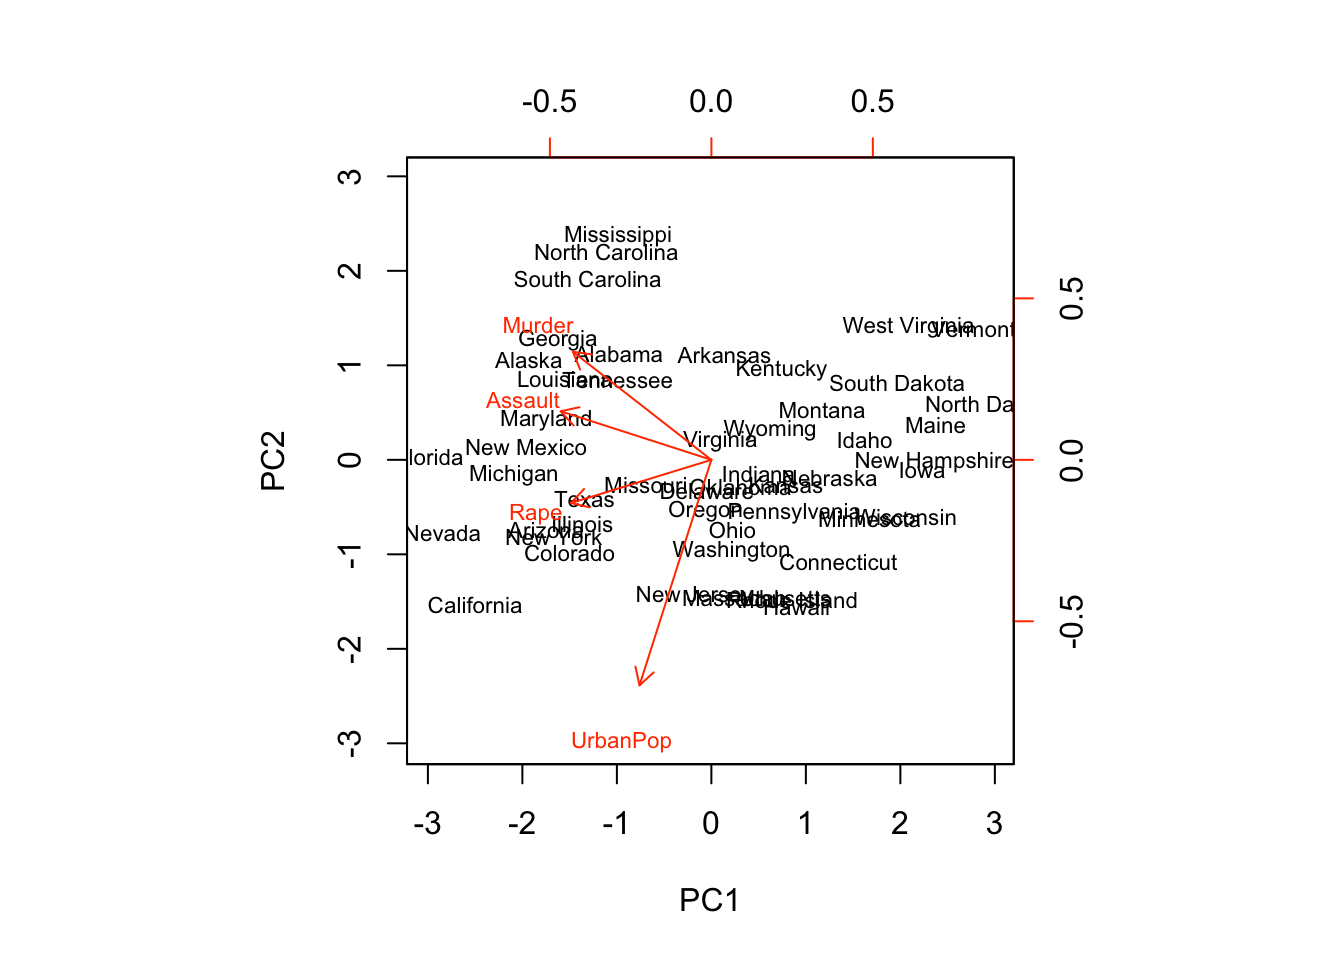
\includegraphics[width=0.7\linewidth]{USAarrests}
	\caption{\textbf{BiPlot}.
		Arrest type data for USA states. 
		Data includes urban population size, number of rape related arrests, assault related, and murder related ($p=4$). 
		Each city is presented against its two first PCs. 
		Arrows encode the loadings. 
		They show that PC1 encodes a general crime level, as it is the average of all type of crimes. 
		PC2 measures the level of urbanization, as it is dominated by the UrbanPopulation variable. 		
		\\ Source: \url{https://goo.gl/85qtKv}}
	\label{fig:usaarrests}
\end{figure}



\subsubsection{Scree Plot}
\label{sec:scree_plot}
[TODO]



\subsection{Mathematics of PCA}
\label{sec:pca_mathematics}
We now present the derivation of PCA from the two different motivations.

\subsubsection{Variance Maximizing View of PCA}

\begin{proof}
	The sketch of the proof is the following:
	We will first show that the weight vector that maximizes the variance is the eigenvector that corresponds to the first principal component.
	We will do so for the \emph{population} covariance, $\Sigma$, and wrap up by plugging its empirical counterpart, $X'X$ (assuming a centered $X$). 
		
	Starting with the first principal component.
	For a random $p$-vector, $\x$ denote $\Sigma:=\cov{\x}$, so that for a fixed $p$-vector $v$: $\cov{v'\x}=v' \Sigma v$.
	Finding a linear combination of $\x$ that best separates individuals, means maximizing $\cov{v'x}$
	w.r.t. to $v$.
	Clearly, $\cov{v'x}$ may explode if any $v$ is allowed. 
	It is most convenient, mathematically, to constrain the $l_2$ norm: $\normII{v}^2=1$.
	Maximizing under a constraint, using Lagrange-Multipliers: 
	\begin{align}
	\argmax{v}{v' \Sigma v - \lambda (\normII{v}^2-1)}.
	\end{align}
	Differentiating w.r.t $v$ and equating zero: 
	\begin{align}
	(\Sigma- \lambda I) v = 0
	\end{align}
	We thus see that any of the $p$ eigenvalue-eigenvector pairs of $\Sigma$ is a local extremum. 
	Which of them to pick?
	To find a \emph{global} maximum we return to the original problem, as plug our result:
	\begin{align}
	\label{eq:pca_maximal_variance}
	\argmax{v:\normII{v}^2=1}{v' \Sigma v }=\argmax{\lambda}{v' \lambda v }
	\end{align}
	so that the global maximum is obtained with the largest eigen-value $\lambda$.
	Put differently, the weight vector that returns the score that best separates individuals, is the eigenvector of $\Sigma$ with the largest eigenvalue. 
	
	The second principal component can be found by solving the same problem, with the additional constraint of $v_2$ orthogonal to $v_1$.
	
	The last missing ingredient is that instead of the true covariance between the features, $\Sigma$, we use the (centered) empirical covariance $X'X$.
\end{proof}


\begin{remark}
Readers familiar with matrix norms will recognize that the above is exactly the derivation of the spectral norm of $\Sigma$.
\end{remark}



\subsubsection{Linear-Space approximation view}

In here, we try to find a series of $\manifold_q; q=1,\dots,p$, such that $\manifold_q$ is a \emph{linear} subspace of dimension $q$ which well approximates $X$ in some (matrix) norm. 
For the deatils, see for instance \cite{shalev2014understanding}.




\subsubsection{Why did Hotelling and Pearson arrive to the same solution?}
\label{sec:pca_intuition}

We have currently offered two motivations for PCA: 
(i) Find linear combinations $v_1,\dots,v_p$ that best distinguish between observations, i.e., maximize variance. 
(ii) Find the linear subspaces $\manifold_1,\dots,\manifold_p$ that best approximates the data.
The reason these two problems are equivalent, is due to the use of the squares-error/Euclidean norms.

Informally speaking, the data has some total variance. 
In analogy to the $SST=SSR+SSE$ decomposition in linear regression, the total variance of $X$ can be decomposed into the part in $\manifold_q$, and the part orthogonal. 
The orthogonal part is the distance of $X$ from $\manifold_q$. 
Maximizing the variance in $\manifold_q$ is thus the same as minimizing the distance from $X$ to $\manifold_q$. 

The only unresolved matter- is why the solution to the variance maximization problem is a \emph{linear} subspace?
This is simply because all the scores, are linear combinations of columns of $X$, thus span a linear subspace, as is sought in the linear-subspace approximation view. 


\subsection{How many PCs can you recover?}
On the face of it, with $p$ variables you can find $p$ PCs. 
Things are not that simple however.

In the population version of the problem, i.e., when $\Sigma$ is known, there may be as many non zero eigenvalues as the rank of $\Sigma$. 
Stating that $\Sigma$ is full rank, is stating that the variables of $\x$ are not fully correlated.

In the empirical version of the problem, i.e., when $X'X$ is known, there may be as many non zero eigenvalues as the rank of $X'X$.
Clearly, if $p>n$, variables of $X$ have to be linearly dependent, so that $X'X$ cannot possibly be of full rank.
To say that the kernel of $X$ is of rank $p-n>0$, is to say that there are $p-n$ scores that are identically zero, thus have no variance. 


Problems do not end when $p<n$. 
This is because if $p<n$ but $p\sim n$ then we do not have many observations per estimated parameter. 
In the statistical literature, this is known as a \emph{high dimensional} problem. 
In the engineering parlance, we say we have low \emph{signal to noise}.
For a rigorous treatment of the statistical properties of PCA, see \cite{nadler2008finite}.
 





\subsection{PCA as a Graph Method}
\label{remark:pca_as_graph}

It turns out that we may find the sequence of best approximating linear subspaces, i.e., the PCs, without the actual measurements $X$, but only with a dissimilarity graph. 
In particular, with the $n\times n$ graph $\dissimilaritys$ of Euclidean distances between individuals: $\dissimilaritys_{i,j}:= \normII{x_i-x_j}$. 

It should come of no surprise that we done need the actual measurements, $X$, since the optimal loadings, $v$, only depend on the covariance $\Sigma$, or its empirical counterpart, $X'X$. 
It may, however, be quite surprising that given the distances between individuals, we may not recover the covariance between variables, $X'X$, but we can recover the PCs. 
Put differently, to find the low dimensional $\manifold$ that approximates the data, we don't need the whole data, but rather, only the graph of distances between data points. 

For proof of the above statement, we refer the reader to \cite[Sec.18.5.2]{friedman2001elements}

This observation will later be very useful for other dimensionality reduction algorithms, which operate not on the original data points, but rather, on dissimilarity graphs. 





\section{Preliminaries}

\subsection{Terminology}

\begin{tcolorbox}
	\begin{description}
		
		\item[Variable] \Aka \emph{dimension}, or \emph{feature} in the machine learning literature, or \emph{column} for reasons that will be obvious in the next item. 
		
		\item[Data] \Aka \emph{sample}, \emph{observations}, depending on your community. 
		Will typically consist of $n$, $p$ dimensional vectors, i.e., with $p$ variables in each.
		We typically denote the data as a $n\times p$ matrix $X$. 
		
		\item[Manifold] A space which is regular enough so that it is \emph{locally} has all the properties of a linear space. 
		We will denote an arbitrary manifold by $\manifold$.
		
		
		\item[Embedding] Informally speaking: a ``shape preserving'' mapping of a space into another. 
		
		\item[Linear Embedding] An embedding done via a linear operation (thus representable by a matrix). 
		
		\item[Generative Model] Known to statisticians as the \emph{sampling distribution}. 
		The assumed stochastic process that generated the observed data. 
		
	\end{description}
\end{tcolorbox}




\subsection{Motivations}
\begin{enumerate}
	\item Scoring (Hotelling motivation).
	\item Recovering latent signal (Blind signal reconstruction).
	\item Improving SNR (before supervised learning).
	\item Decreasing computational complexity. 
\end{enumerate}


\subsection{Taxonomy }
\begin{enumerate}
	\item Linear $\manifold$ vs. non-linear manifold. 
\end{enumerate}





\section{Purely Algorithmic Approaches}




\section{Generative Approaches}



\section{Dealing with the high-dimension}






\newpage
\bibliographystyle{abbrvnat}
\bibliography{dim_reduce.bib}



\end{document}
